\documentclass[12pt]{article}

\usepackage{sbc-template}

\usepackage{graphicx,url}

\usepackage[brazil]{babel}
%\usepackage[latin1]{inputenc}
\usepackage[utf8]{inputenc}
% UTF-8 encoding is recommended by ShareLaTex


\sloppy

\title{Análise de Simulações \textit{in silico} do Crescimento de Tumores Malignos em Nível Celular}

\author{Arthur Passos\inst{1}, Halersson Paris Goes\inst{1}, Fernando Concatto\inst{1}}

\address{Universidade do Vale do Itajaí (UNIVALI)\\
  Caixa Postal 360 -- CEP 88302-202 -- Itajaí -- SC -- Brasil
  \email{\{arthur.titel,halersson,fernandoconcatto\}@gmail.com}
}

\begin{document}

\maketitle

\begin{abstract}
  This meta-paper describes the style to be used in articles and short papers
  for SBC conferences. For papers in English, you should add just an abstract
  while for the papers in Portuguese, we also ask for an abstract in
  Portuguese (``resumo''). In both cases, abstracts should not have more than
  10 lines and must be in the first page of the paper.
\end{abstract}

\begin{resumo}
  O câncer é uma das principais causas de morte em diversos países, e prevê-se que o número de novos casos aumentará significativamente no futuro próximo. Neste contexto, a modelagem matemática da doença fornece uma plataforma para a realização de experimentações e a descoberta de novos conhecimentos quanto à seu comportamento através de meios computacionais, contornando a necessidade de utilização de materiais orgânicos. Assim, este trabalho buscou investigar modelos matemáticos de crescimento de tumores malignos, analisando-os tanto em relação à sua expressividade quanto à sua capacidade de representar fielmente o fenômeno real, levando em conta a construção de um simulador de fácil compreensão. % concluir melhor? Está bem abstrato
\end{resumo}

\section{Introdução}

O grupo de doenças conhecido como câncer é caracterizado pelo crescimento desinibido de células anormais em um organismo, possuindo a capacidade de invadir o sistema circulatório e se espalhar para órgãos distantes. Diversos fatores podem causar o surgimento do câncer, incluindo tanto hábitos e o estilo de vida individual quanto características genéticas. Mundialmente, o câncer (também chamado de tumor maligno ou neoplasia) é a segunda causa mais frequente de morte, sendo responsável pelo falecimento de aproximadamente 9 milhões de indivíduos no ano de 2015 \cite{WHO2017,ACS2017}.

Para um melhor entendimento do câncer, foram propostas seis características biológicas que juntas formam o princípio da diversidade de doenças neoplásicas, tais características são adquiridas progressivamente durante o desenvolvimento do tumor, elas são denominadas: autossuficiência em sinais estimuladores de crescimento (\emph{Sustaining Proliferative Signaling}), evasão de supressores de crescimento (\emph{Evading Growth Suppressors}), resistência a mecanismos naturais de morte celular (\emph{Resisting Cell Death}), potencial ilimitado de multiplicação (\emph{Enabling Replicative Immortality}), estimulo a angiogenesis (\emph{Inducing Angiogenesis}) e a invasão de outros tecidos e capacidade de fazer metástases.
stemas que regulam e limitam o crescimento celular.
ancerigênas podem desenvolver vários mecânismos para limitar ou até mesmo dibrar este processo. O método mais comum é através da perda da função TP53, outra forma é através do aumento de reguladores antiapoptoticos.



Potencial ilimitado de multiplicação: 





%http://www.cell.com/cell/fulltext/S0092-8674(11)00127-9, https://drfelipeades.wordpress.com/2014/11/13/as-seis-principais-caracteristicas-do-cancer/



% Falar sobre as características do câncer. Ver Hallmarks of Cancer.

% Falar sobre experimentações in vivo e as dificuldades. Ver Cancer Modeling and Simulation (e-mail Santana)
Um ciclo ideal para afirmações do desenvolvimento citado nas pesquisas, faz-se necessário observações fenomenológicas, na qual toda teoria relatada é alterada para experiências de consciência. Cientistas em medicina biológica optam por abordagens inofensivas, onde são realizadas testes in vivo, ou seja, ratos, embriões de frangos ou in vitro. Os resultados das experiência observáveis, tanto por meios biológicos, matemáticos ou físicos, podem gerar modelos à fins de descrever comportamentos padrões.




% Falar sobre modelagem matemática em geral e de câncer. Ver artigos de survey

% Aprofundar para o contexto do artigo, falando sobre o objetivo e apresentar seções (separar parágrafos se ficar grande).

\section{Revisão bibliográfica} % Alt: Trabalhos relacionados

% Falar sobre alguns artigos relacionados, não necessariamente aqueles que acabamos utilizando. Citar outras abordagens além de equações diferenciais. Falar sobre crescimento logístico/Gompertz, etc. MUITAS citações nesta seção.

\section{Metodologia} % Alt: Modelos e métodos

% Aprofundar em relação aos modelos utilizados. Apresentar as equações detalhadamente, trazendo paralelos com a seção passada

% Falar sobre discretização e o método de Euler (podemos pensar em Diferenças Finitas pra ter uma comparação)

\section{Análise de resultados}

% Muitas tabelas e gráficos. Falar sobre semelhanças e diferenças. Comparar, analisar, descrever

\section{Conclusões}

% Falar brevemente sobre tudo que fizemos.

% O que descobrimos? Falar sobre os pontos positivos e negativos da abordagem

% Apresentar sugestões para trabalhos futuros.

All full papers and posters (short papers) submitted to some SBC conference,
including any supporting documents, should be written in English or in
Portuguese. The format paper should be A4 with single column, 3.5 cm for upper
margin, 2.5 cm for bottom margin and 3.0 cm for lateral margins, without
headers or footers. The main font must be Times, 12 point nominal size, with 6
points of space before each paragraph. Page numbers must be suppressed.

Full papers must respect the page limits defined by the conference.
Conferences that publish just abstracts ask for \textbf{one}-page texts.

\section{First Page} \label{sec:firstpage}

The first page must display the paper title, the name and address of the
authors, the abstract in English and ``resumo'' in Portuguese (``resumos'' are
required only for papers written in Portuguese). The title must be centered
over the whole page, in 16 point boldface font and with 12 points of space
before itself. Author names must be centered in 12 point font, bold, all of
them disposed in the same line, separated by commas and with 12 points of
space after the title. Addresses must be centered in 12 point font, also with
12 points of space after the authors' names. E-mail addresses should be
written using font Courier New, 10 point nominal size, with 6 points of space
before and 6 points of space after.

The abstract and ``resumo'' (if is the case) must be in 12 point Times font,
indented 0.8cm on both sides. The word \textbf{Abstract} and \textbf{Resumo},
should be written in boldface and must precede the text.

\section{CD-ROMs and Printed Proceedings}

In some conferences, the papers are published on CD-ROM while only the
abstract is published in the printed Proceedings. In this case, authors are
invited to prepare two final versions of the paper. One, complete, to be
published on the CD and the other, containing only the first page, with
abstract and ``resumo'' (for papers in Portuguese).

\section{Sections and Paragraphs}

Section titles must be in boldface, 13pt, flush left. There should be an extra
12 pt of space before each title. Section numbering is optional. The first
paragraph of each section should not be indented, while the first lines of
subsequent paragraphs should be indented by 1.27 cm.

\subsection{Subsections}

The subsection titles must be in boldface, 12pt, flush left.

\section{Figures and Captions}\label{sec:figs}


Figure and table captions should be centered if less than one line
(Figure~\ref{fig:exampleFig1}), otherwise justified and indented by 0.8cm on
both margins, as shown in Figure~\ref{fig:exampleFig2}. The caption font must
be Helvetica, 10 point, boldface, with 6 points of space before and after each
caption.

\begin{figure}[ht]
\centering
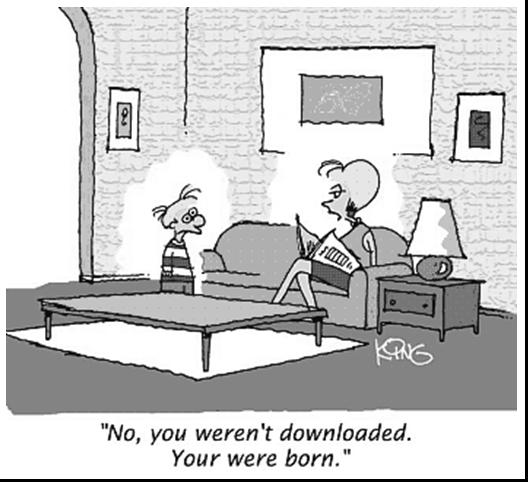
\includegraphics[width=.5\textwidth]{fig1.jpg}
\caption{A typical figure}
\label{fig:exampleFig1}
\end{figure}

\begin{figure}[ht]
\centering
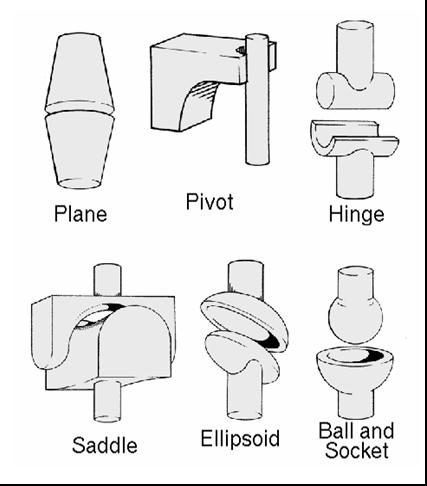
\includegraphics[width=.3\textwidth]{fig2.jpg}
\caption{This figure is an example of a figure caption taking more than one
  line and justified considering margins mentioned in Section~\ref{sec:figs}.}
\label{fig:exampleFig2}
\end{figure}

In tables, try to avoid the use of colored or shaded backgrounds, and avoid
thick, doubled, or unnecessary framing lines. When reporting empirical data,
do not use more decimal digits than warranted by their precision and
reproducibility. Table caption must be placed before the table (see Table 1)
and the font used must also be Helvetica, 10 point, boldface, with 6 points of
space before and after each caption.

\begin{table}[ht]
\centering
\caption{Variables to be considered on the evaluation of interaction
  techniques}
\label{tab:exTable1}
\smallskip
\begin{tabular}{|l|c|c|}
\hline
& Value 1 & Value 2\\[0.5ex]
\hline
&&\\[-2ex]
Case 1 & 1.0 $\pm$ 0.1 & 1.75$\times$10$^{-5}$ $\pm$ 5$\times$10$^{-7}$\\[0.5ex]
\hline
&&\\[-2ex]
Case 2 & 0.003(1) & 100.0\\[0.5ex]
\hline
\end{tabular}
\end{table}

\section{Images}

All images and illustrations should be in black-and-white, or gray tones,
excepting for the papers that will be electronically available (on CD-ROMs,
internet, etc.). The image resolution on paper should be about 600 dpi for
black-and-white images, and 150-300 dpi for grayscale images.  Do not include
images with excessive resolution, as they may take hours to print, without any
visible difference in the result.

\section{References}

Bibliographic references must be unambiguous and uniform.  We recommend giving
the author names references in brackets, e.g. \cite{knuth:84},
\cite{boulic:91}, and \cite{smith:99}.

The references must be listed using 12 point font size, with 6 points of space
before each reference. The first line of each reference should not be
indented, while the subsequent should be indented by 0.5 cm.

\bibliographystyle{sbc}
\bibliography{tumorgrowth}

\end{document}
